%%%%%%%%%%%%%%%%%%%%%%%%%%%%%%%%%%%%%%%%%%%%%%%%%%%%%%%%%%%%%%%%%%%%%%%%%%%
% Definitions                                                             %
%%%%%%%%%%%%%%%%%%%%%%%%%%%%%%%%%%%%%%%%%%%%%%%%%%%%%%%%%%%%%%%%%%%%%%%%%%%
\gdef\version{0.1}
\gdef\doctype{Sprint 1}

\documentclass[11pt]{article}
%Gummi|065|=)

\usepackage{eurosym}
\usepackage{listings}
\usepackage{color}
\usepackage[dvipsnames]{xcolor}
\usepackage{graphicx}
\graphicspath{ {.} }
\usepackage{upgreek}
\usepackage{titlesec}
\usepackage{fancyhdr}
\usepackage{tabulary}
\usepackage[utf8]{inputenc}
\usepackage{lastpage}
\usepackage{tikz}
\usepackage{gensymb}


%for code snippets
\lstset{
  language=C,                	  % choose the language of the code
  numbers=left,                   % where to put the line-numbers
  stepnumber=1,                   % the step between two line-numbers.
  numbersep=5pt,                  % how far the line-numbers are from the code
  backgroundcolor=\color{white},  % choose the background color. You must add \usepackage{color}
  showspaces=false,               % show spaces adding particular underscores
  showstringspaces=false,         % underline spaces within strings
  showtabs=false,                 % show tabs within strings adding particular underscores
  tabsize=2,                      % sets default tabsize to 2 spaces
  captionpos=b,                   % sets the caption-position to bottom
  breaklines=true,                % sets automatic line breaking
  breakatwhitespace=true,         % sets if automatic breaks should only happen at whitespace
  title=\lstname,                 % show the filename of files included with \
}

%%%%%%%%%%%%%%%%%%%%%%%%%%%%%%%%%%%%%%%%%%%%%%%%%%%%%%%%%%%%%%%%%%%%%%%%%%%
% Header                                                                  %
%%%%%%%%%%%%%%%%%%%%%%%%%%%%%%%%%%%%%%%%%%%%%%%%%%%%%%%%%%%%%%%%%%%%%%%%%%%
\renewcommand{\headrulewidth}{0.4pt}
\renewcommand{\footrulewidth}{0.4pt}
\renewcommand{\arraystretch}{1.4}
\fancyhead{}
\fancyfoot{}
\pagestyle{fancy}
\lhead{{\doctype}}
\rhead{{\fontfamily{phv}\selectfont \textcolor{gray}{Urban Green}} 
\includegraphics[height=0.8cm]{logo}}
\lfoot{Version \version}
\rfoot{\thepage\ von \pageref{LastPage}}
\setlength{\headheight}{30pt}


%%%%%%%%%%%%%%%%%%%%%%%%%%%%%%%%%%%%%%%%%%%%%%%%%%%%%%%%%%%%%%%%%%%%%%%%%%%
% Document Start                                                          %
%%%%%%%%%%%%%%%%%%%%%%%%%%%%%%%%%%%%%%%%%%%%%%%%%%%%%%%%%%%%%%%%%%%%%%%%%%%
\begin{document}
\begin{titlepage}
    \centering
    \vfill
    {
        \Huge\textbf{Sprint 1}\\
        \vskip2cm
        
\includegraphics[width=4cm]{logo} \\
        \Large
        {\fontfamily{phv}\selectfont
			\textcolor{gray}{Urban Green}
		}
        \vskip3cm
        Matthias Schwebler\\
        Ramin Bahadoorifar\\
        Samuel Schober\\
        Konrad Kelc\\
    }
    \vfill
    \begin{center}
    \begin{table}[ht]
    	\centering
    	\begin{tabular}{lllll}
    		\cline{1-4}
    		\multicolumn{1}{|c|}{\textbf{\rule{0pt}{3ex} }} & \multicolumn{1}{c|}{\textbf{Name}} & \multicolumn{1}{l|}{\textbf{Datum}} & \multicolumn{1}{l|}{\textbf{Unterschrift}} &  \\ \cline{1-4}

    		\multicolumn{1}{|l|}{\textbf{\rule{0pt}{3ex} Erstellt:}} & \multicolumn{1}{l|}{M. Schwebler, R. Bahadoorifar} & \multicolumn{1}{l|}{TT.MM.YYYY} & \multicolumn{1}{l|}{} &  \\ \cline{1-4}

    		\multicolumn{1}{|l|}{\textbf{\rule{0pt}{3ex} Gepr\"uft:}} & \multicolumn{1}{l|}{S. Schober, K. Kelc} & \multicolumn{1}{l|}{TT.MM.YYYY} & \multicolumn{1}{l|}{} &  \\ \cline{1-4}
    		&  &  &  &  \\
    		&  &  &  &  \\
    		&  &  &  &  \\
    	\end{tabular}
    \end{table}
    \end{center}
\end{titlepage}

\tableofcontents	%Inhaltsverzeichnis

\newpage
% Versionierung
\begin{table}[ht]
\centering
\begin{tabular}{|l|l|l|l|l}
\cline{1-4}
\multicolumn{1}{|c|}{\textbf{Datum}} & \multicolumn{1}{c|}{\textbf{Version}} & \multicolumn{1}{c|}{\textbf{Autor}}                                                                               & \multicolumn{1}{c|}{\textbf{Status}} &  \\ \cline{1-4}
TT.MM.YYYY                           & 0.1                                   & \begin{tabular}[c]{@{}l@{}}Matthias Schwebler,\\ Ramin Bahadoorifar,\\ Konrad Kelc,\\ Samuel Schober\end{tabular} & Erstentwurf                          &  \\ \cline{1-4}
TT.MM.YYYY                           & 1.0                                   & \begin{tabular}[c]{@{}l@{}}A B,\\ X Y\end{tabular}                                  & Fertigstellung                       &  \\ \cline{1-4}
TT.MM.YYYY                           & 1.1                                  & \begin{tabular}[c]{@{}l@{}}A B,\\ X Y\end{tabular}                                  & \"Uberarbeitung                       &  \\ \cline{1-4}
\end{tabular}
\end{table}
\newpage
\section{Datenmanagement}
\subsection{Verwaltung der lokalen Daten - User Story 1571 u. 2097}
Um alle Daten der Sensoren Abzulesen wird die Serielle Schnittstelle verwendet. Der C-Code der auf dem Arduino ausgef\"uhrt wird, sendet alle Informationen an den Raspberry Pi. Dieser muss lediglich auf der Schnittstelle auf eingehende Daten warten, was mit einem Python Script realisiert wird. Hierbei werden die Libraries "redis", "serial" und "time" verwendet. Damit es zu keinen Problemen beim Auslesen kommt, muss nach jedem Lesevorgang 0.1 Sekunden pausiert werden. Falls dies nicht eingehalten wird, wird beispielsweise "temperature" zu "temp" und "erature". Der folgende Code ist ein Beispiel, wie dauerhaft Daten ausgelesen und in die Datenbank gespeichert werden k\"onnen.
\begin{lstlisting} [language=Python, frame=single]
import redis
import serial
import time

# init serial
# TODO 'ttyACM0' needs to be changed to whatever the raspberry Pi's USB-port is called
ser = serial.Serial(
	port='/dev/ttyACM0',
	baudrate=115200
)
# init redis
r = redis.StrictRedis(host='localhost', port=6380, db=0)

data = ""
while True:
	bytesToRead = ser.inWaiting()
	data = ser.read(bytesToRead)
	if data != "":
		kv = data.split(' ',data)   # kv... KeyValue
		r.hset('system', kv[0], kv[1])   # write data to redis
		time.sleep(0.1)
\end{lstlisting}

\subsection{\"Ubertragung zum zentralen Server - User Story 1984}
Um die lokal gespeicherten Daten zum zentralen Server zu \"ubertragen, wird wieder ein Python Script verwendet. Da auf dem Server MongoDB verwendet wird, muss zuerst auf dem lokalen SBC die entsprechende Library installiert werden. Dies geschieht mit folgendem Befehl:
\begin{lstlisting} [frame=single]
pip install pymongo	
\end{lstlisting}
Im Python Script muss zuerst die Verbindung zu den beiden Datenbanken hergestellt werden:
\begin{lstlisting} [language=Python, frame=single]
# init mongodb and redis
mongoClient = MongoClient('vps336521.ovh.net', 27017)
r = redis.StrictRedis(host='localhost', port=6380, db=0)

# get database
db = mongoClient.urbangreen

# get collection
collection = db['sensor-data']
\end{lstlisting}
Danach kann mit folgendem Code ein neuer Datensatz angelegt werden:
\begin{lstlisting} [language=Python, frame=single]
newData = {
	"temperature": r.hget("system", "temperature"),
	"ph": r.hget("system", "ph"),
	"ec": r.hget("system", "ec")
}
collection.insert_one(newData)
\end{lstlisting}

\newpage
\section{Aktoren}
\subsection{Hitestrahler - User Story 1583}
Um die Temperatur zu regeln, wird der Hitzestrahler von cooking-hacks.com verwendet. Er kann in einen der fünf dafür vorgesehenen Slots mit dem OpenAquarium Shield für den Arduino verbunden werden. Der Hitzestrahler kann jeweils mit einer einzigen Code Zeile ein- bzw. ausgeschaltet werden.
\begin{lstlisting} [language=C, frame=single]
	OpenAquarium.sendPowerStrip(on1); 
	OpenAquarium.sendPowerStrip(off1);
\end{lstlisting}
"on1" und "off1" sind konstanten die von cooking-hacks.com vorgegeben sind.
Dieser Code funktioniert, solange der Hitzestrahler auf dem ersten Socket angeschlossen ist. Angenommen er wäre mit dem zweiten Socket verbunden müsste "on2" und "off2" verwendet werden. \\
Um beispielsweise die Temperatur zwischen 25 und 27 Grad Celsius zu halten würde folgender Code ausreichen:
\begin{lstlisting} [language=C, frame=single]
  if(temperature<25){ 
    OpenAquarium.sendPowerStrip(on1)
  }
  if(temperature>27){ 
    OpenAquarium.sendPowerStrip(off1);
  }
\end{lstlisting}
Kenndaten des Hitzestrahlers:
\begin{itemize}
\item Leistung: 100W
\item Spannung: 220/240V 50/60Hz
\item Temperatur: 17\degree C - 23\degree C
\end{itemize}

\newpage
\section{Sensoren}
\subsection{Wasserstand - User Story 2083}
Es ist wichtig den Wasserstand regelmäßig zu prüfen, da das System oft lange Zeit unbeaufsichtig bleibt. Wenn zu viel Wasser verdunstet muss es nachgefüllt werden. Hierfür wird der Wasserstandsensor von cooking-hacks.com verwendet. Er kann auf dem OpenAquarium Board angeschlossen werden und über die entsprechende Library angesprochen werden. \\
\begin{minipage}{5in}
  \centering
  \raisebox{-0.5\height}{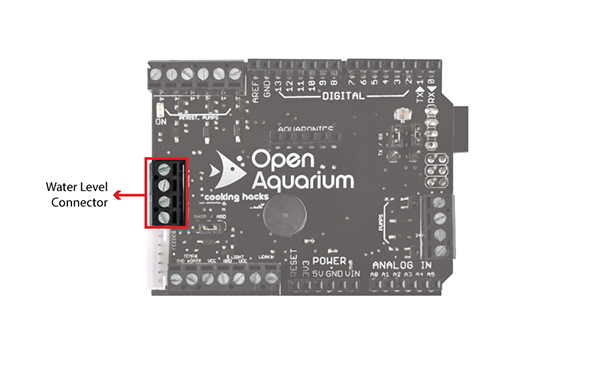
\includegraphics[height=3.0in]{waterLevel_connection}}
\end{minipage}
Abfragen des Wasserstands:
\begin{lstlisting} [language=C, frame=single]
OpenAquarium.waterlevel1();
\end{lstlisting}
Die Methode "waterlevel1()" testet automatisch den Wasserstand und schreibt auf die Serielle schnittstelle den aktuellen Status ("Aquarium Full"/"Aquarium Empty")
\end{document}
